%!TEX program = xelatex
\documentclass[11pt,utf8]{article}
\usepackage[no-math]{fontspec}
\usepackage{amsmath}
\usepackage{amsthm}
\usepackage{amssymb}
%\usepackage{xeCJK}
\usepackage{verbatim}
\usepackage{indentfirst}
\usepackage{syntonly}
\usepackage{fancyhdr}
\usepackage[unicode=true, colorlinks, linkcolor=black, anchorcolor=black, citecolor=black, urlcolor=black]{hyperref}
\usepackage{graphicx}
\usepackage[top = 1.2in, bottom = 1.2in, left = 1.3in, right = 1.3in]{geometry}
\usepackage[svgnames]{xcolor}
\usepackage{paralist}
\usepackage{ulem}
\usepackage{titlesec}
\usepackage{zhspacing}
\usepackage{booktabs}
\usepackage{multirow}
\usepackage{multicol}
\usepackage{supertabular}
\usepackage[final]{pdfpages}
\usepackage{mdframed}
\usepackage{longtable}

\defaultfontfeatures{Mapping=tex-text}
\zhspacing
%\setromanfont{Computer Modern Roman}
\newfontfamily\zhfont{Songti SC}
\setmonofont[Scale=1]{Courier New}
\XeTeXlinebreaklocale "zh"
\XeTeXlinebreakskip = 0pt plus 1pt

\pagestyle{fancy}
\pagestyle{plain}

\begin{document}
	
	\newcommand{\hlink}[1]{
		\footnote{\href{#1}{\textsl{\underline{#1}}}}
	}
	\renewenvironment{proof}{\noindent{\textbf{证明:}}}{\hfill $\square$ \vskip 4mm}
	\newtheorem*{theorem*}{定理}
	\newcommand{\theorem}[1]{
		\begin{theorem*}\textup{#1}\end{theorem*}
	}
	\let\enumerate\compactenum
	\let\endenumerate\endcompactenum
	\let\itemize\compactitem
	\let\enditemize\endcompactitem
	\setlength{\pltopsep}{5pt}
	\setlength{\parindent}{2em}
	\setlength{\footskip}{30pt}
	\setlength{\baselineskip}{1.3\baselineskip}
	\renewcommand\arraystretch{1.2}
	
	\colorlet{LightGray}{Gray!10!}
	
	\begin{titlepage}
		\fancyhead[CH]{}
		
		\hspace{3.0cm}
		\begin{center}
			\vfill
			% Upper part of the page
			
			\textsc{\LARGE Tsinghua University}\\[0.8cm]
			
			\textsc{\Large Computer Organization Experimentation}\\[2.5cm]
			
			
			% Title
			\rule[0.75\baselineskip]{0.75\textwidth}{1pt}
			
			{ \huge \bfseries Project Test Document}\\[0.4cm]
			
			\rule[15\baselineskip]{0.75\textwidth}{1pt}
			
			% Author and supervisor
			\begin{minipage}{0.4\textwidth}
				\begin{flushleft} \large
					\emph{Author:}\\
					Shizhi \textsc{Tang}
					
					Xihang \textsc{Liu}
					
					Zixi \textsc{Cai}
				\end{flushleft}
			\end{minipage}
			\begin{minipage}{0.4\textwidth}
				\begin{flushright} \large
					\emph{Supervisor:} \\
					Yuxiang \textsc{Zhang}
					
					Prof.~Weidong \textsc{Liu}
				\end{flushright}
			\end{minipage}
			
			\vfill
			\vspace{3.0cm}
			% Bottom of the page
			{\large \today}
			
		\end{center}
		
	\end{titlepage}
	\renewcommand{\headrulewidth}{0.4pt}
	\setcounter{page}{2}
	\tableofcontents
	\newpage
	

\section{单元测试} {

\subsection{框架说明} {
在开发的初期实现的指令尚不完全的时候,无法覆盖功能测试所必须的指令,然而我们又必须对我们实现的指令进行单元测试,以减少后续集成测试的难度。于是我们自己开发了一个简单易用的单元测试框架。这个框架使用过程是:编写一个非常直观的testcase文件,经过build之后可以转换成为.vhd格式的仿真文件;将生成的仿真文件加入到Vivado中,便可对这个testcase进行测试。除了在仿真时观察波形以检查执行过程的正确性外,我们提供了更为简洁的选择:在testcase文件中可以通过ASSERT对某个时刻某个寄存器(或是其他信号)的值进行断言。这种方式能够将我们对测试结果的检查聚焦在我们所关心的对象上,比起波形也更加具有可读性,能更好地发现问题,从而更高效地迭代。以下展示了一个testcase文件的示例,其中包含了对testcase文件语法的说明。
\begin{table}[!htb]
	\begin{center}
		\begin{tabular*}{15cm}{lll}  
			\hline  
\# 单行注释以\#开头\\
\\
\# 导入一个package\\
\# 语法: "IMPORT <package名称>"\\
IMPORT alu\_const\\
\\
\# 定义一个要检查的信号\\
\# 语法: "DEFINE <定义信号名> <元件实例名1.元件实例名2.(...).原信号名>: <信号类型>"\\
DEFINE reg regfile\_ist.regArray: RegArrayType\\
\\
\# 执行一条汇编指令\\
\# 语法: "RUN <指令>"\\
RUN ori \$2, \$0, 0x0020\\
\\
\# 对某个之前定义的信号的值进行断言
\# 语法: "ASSERT <周期号> <信号名> <值>"\\
\# 第0个周期是重启后一开始的周期\\
ASSERT 6 reg(2) x"20000234"\\
\\
RUN ori \$2, \$3, 0xffff\\
ASSERT 7 reg(2) x"00000000"\\
\\
RUN ori \$2, \$4, 0xfffe\\
			\hline  
		\end{tabular*}  
	\end{center}
\end{table}

可以看到,testcase可读性非常好,写起来自然,且方便维护。
}

\subsection{逻辑运算与移位运算指令} {
\subsubsection{测试对象} {
逻辑运算指令:ori、andi、xori、or、and、xor、nor。

移位运算指令:sll、sllv、srl、srlv、sra、srav。

加载立即数指令:lui。

0号寄存器的处理。

数据相关问题的处理。
}
\subsubsection{测试思路} {
执行要测试的逻辑运算和移位运算指令,在每条逻辑运算指令执行完毕的时间节点ASSERT目的寄存器的预期结果。为了验证0号寄存器的处理是否正确,测试要涵盖源寄存器为0号寄存器和目的寄存器为0号寄存器的情况。为了验证对立即数的扩展都是无符号扩展,对把立即数当做操作数的指令需要设计立即数的最高位是1的情况。

为了验证数据相关的处理是否正确,需要设计三种情况,即在某一条语句之后的第一条、第二条、第三条语句中把该语句的目的寄存器作为源寄存器。
}
\subsubsection{testcase} {
注意:所有的testcase文件的注释和空行都已删除(下同)。
\begin{center}	\begin{longtable}{p{15cm}} \hline
		IMPORT{ }global\_const\\
		DEFINE{ }reg{ }regfile\_ist.regArray:{ }RegArrayType\\
		RUN{ }ori{ }\$2,{ }\$0,{ }0x0020\\
		ASSERT{ }6{ }reg(2){ }32ux"0020"\\
		RUN{ }ori{ }\$0,{ }\$2,{ }0xffff\\
		ASSERT{ }7{ }reg(0){ }32ux"0000"\\
		RUN{ }ori{ }\$3,{ }\$2,{ }0x1214\\
		ASSERT{ }8{ }reg(3){ }32ux"1234"\\
		\hline \end{longtable} \end{center}
\begin{center}	\begin{longtable}{p{15cm}} \hline
		RUN{ }ori{ }\$2,{ }\$0,{ }0x1234\\
		RUN{ }ori{ }\$3,{ }\$2,{ }0x2345\\
		RUN{ }ori{ }\$4,{ }\$2,{ }0x3456\\
		RUN{ }ori{ }\$0,{ }\$3,{ }0xffee\\
		RUN{ }ori{ }\$4,{ }\$0,{ }0x4321\\
		\hline \end{longtable} \end{center}
\begin{center}	\begin{longtable}{p{15cm}} \hline
		DEFINE{ }reg{ }regfile\_ist.regArray:{ }RegArrayType\\
		RUN{ }ori{ }\$1,{ }\$2,{ }0x1234\\
		ASSERT{ }6{ }reg(1){ }32ux"1234"\\
		RUN{ }xori{ }\$3,{ }\$1,{ }0x8921\\
		ASSERT{ }7{ }reg(3){ }32ux"9b15"\\
		RUN{ }andi{ }\$4,{ }\$1,{ }0x4fe2\\
		ASSERT{ }8{ }reg(4){ }32ux"0220"\\
		RUN{ }andi{ }\$5,{ }\$1,{ }0x6543\\
		ASSERT{ }9{ }reg(5){ }32ux"0000"\\
		RUN{ }xori{ }\$3,{ }\$3,{ }0xfeef\\
		ASSERT{ }10{ }reg(3){ }32ux"65fa"\\
		RUN{ }ori{ }\$0,{ }\$5,{ }0xffff\\
		ASSERT{ }11{ }reg(0){ }32ux"0000"\\
		RUN{ }andi{ }\$3,{ }\$0,{ }0x8888\\
		ASSERT{ }12{ }reg(3){ }32ux"0000"\\
		RUN{ }xori{ }\$2,{ }\$0,{ }0x3333\\
		ASSERT{ }13{ }reg(2){ }32ux"3333"\\
		RUN{ }ori{ }\$1,{ }\$0,{ }0x6666\\
		ASSERT{ }14{ }reg(1){ }32ux"6666"\\
		\hline \end{longtable} \end{center}
\begin{center}	\begin{longtable}{p{15cm}} \hline
		IMPORT{ }alu\_const\\
		DEFINE{ }reg{ }regfile\_ist.regArray:{ }RegArrayType\\
		RUN{ }ori{ }\$3,{ }\$0,{ }0x1200\\
		ASSERT{ }6{ }reg(3){ }x"00001200"\\
		RUN{ }ori{ }\$3,{ }\$3,{ }0x00f2\\
		ASSERT{ }7{ }reg(3){ }x"000012f2"\\
		RUN{ }ori{ }\$2,{ }\$0,{ }0x30de\\
		ASSERT{ }8{ }reg(2){ }x"000030de"\\
		RUN{ }or{ }\$6,{ }\$2,{ }\$3\\
		ASSERT{ }9{ }reg(6){ }x"000032fe"\\
		RUN{ }xor{ }\$5,{ }\$2,{ }\$3\\
		ASSERT{ }10{ }reg(5){ }x"0000222c"\\
		RUN{ }nor{ }\$7,{ }\$2,{ }\$3\\
		ASSERT{ }11{ }reg(7){ }x"ffffcd01"\\
		\hline \end{longtable} \end{center}
\begin{center}	\begin{longtable}{p{15cm}} \hline
		IMPORT{ }alu\_const\\
		DEFINE{ }reg{ }regfile\_ist.regArray:{ }RegArrayType\\
		RUN{ }ori{ }\$3,{ }\$0,{ }0x1200\\
		ASSERT{ }6{ }reg(3){ }x"00001200"\\
		RUN{ }ori{ }\$3,{ }\$3,{ }0x00f2\\
		ASSERT{ }7{ }reg(3){ }x"000012f2"\\
		RUN{ }ori{ }\$2,{ }\$0,{ }0x30de\\
		ASSERT{ }8{ }reg(2){ }x"000030de"\\
		RUN{ }or{ }\$6,{ }\$2,{ }\$3\\
		ASSERT{ }9{ }reg(6){ }x"000032fe"\\
		RUN{ }or{ }\$5,{ }\$2,{ }\$3\\
		ASSERT{ }10{ }reg(5){ }x"000032fe"\\
		RUN{ }xor{ }\$5,{ }\$5,{ }\$3\\
		ASSERT{ }11{ }reg(5){ }x"0000200c"\\
		RUN{ }nor{ }\$7,{ }\$2,{ }\$3\\
		ASSERT{ }12{ }reg(7){ }x"ffffcd01"\\
		\hline \end{longtable} \end{center}
\begin{center}	\begin{longtable}{p{15cm}} \hline
		IMPORT{ }alu\_const\\
		DEFINE{ }reg{ }regfile\_ist.regArray:{ }RegArrayType\\
		RUN{ }ori{ }\$3,{ }\$0,{ }0xf200\\
		ASSERT{ }6{ }reg(3){ }x"0000f200"\\
		RUN{ }ori{ }\$2,{ }\$0,{ }0x0010\\
		ASSERT{ }7{ }reg(2){ }x"00000010"\\
		RUN{ }sll{ }\$4,{ }\$3,{ }0x10\\
		ASSERT{ }8{ }reg(4){ }x"f2000000"\\
		RUN{ }srl{ }\$5,{ }\$4,{ }0x10\\
		ASSERT{ }9{ }reg(5){ }x"0000f200"\\
		RUN{ }sra{ }\$5,{ }\$4,{ }0x10\\
		ASSERT{ }10{ }reg(5){ }x"fffff200"\\
		RUN{ }sllv{ }\$4,{ }\$3,{ }\$2\\
		ASSERT{ }11{ }reg(4){ }x"f2000000"\\
		RUN{ }srlv{ }\$5,{ }\$4,{ }\$2\\
		ASSERT{ }12{ }reg(5){ }x"0000f200"\\
		RUN{ }srav{ }\$5,{ }\$4,{ }\$2\\
		ASSERT{ }13{ }reg(5){ }x"fffff200"\\
		\hline \end{longtable} \end{center}

}
}

\subsection{算术运算指令} {
\subsubsection{测试对象} {
加减法指令:add、addu、addiu、sub、subu。

乘法指令:mul、mult、multu。

乘累加乘累减指令:madd、maddu、msub、msubu。

除法指令:div、divu。

其他算术运算指令:slt、sltu、slti、sltiu、clo、clz。

HI、LO寄存器的实现。

流水线暂停的实现。

overflow异常的实现。
}
\subsubsection{测试思路} {
同样分别执行要测试的算术运算指令并通过ASSERT检验结果的正确性。

对于加减法指令,都有检测溢出异常的版本和忽略溢出的版本。在测试检测溢出异常的版本(add、sub)时,一来要验证确实跳转到了异常处理代码(放置在某个固定入口处),二来要验证运算溢出后,运算结果不会写入目的寄存器中。当然也要确保没有溢出的运算正确地将结果写入了目的寄存器,由此确保溢出判断的正确性。

对于除了mul以外的乘法指令、乘累加指令、乘累减指令、除法指令,都会将结果写入HI、LO寄存器。为了验证正确性,需要检查HI、LO寄存器的值是否符合预期。这也同时验证了HI、LO寄存器实现的正确性。

不同于逻辑运算指令,操作数其中之一为立即数的算术运算指令对立即数有符号扩展和无符号扩展两种方式,需要分别进行测试,测试要涵盖立即数最高位为1的情况,以此正确地对立即数扩展进行验证。

乘累加乘累减指令和除法指令运行周期数都大于1,ASSERT的时候要算好时钟周期。这同时也测试了流水线暂停实现的正确性。
}
\subsubsection{testcase} {
\begin{center}	\begin{longtable}{p{15cm}} \hline
		DEFINE{ }reg{ }regfile\_ist.regArray:{ }RegArrayType\\
		RUN{ }ori{ }\$2,{ }\$2,{ }0x33\\
		RUN{ }clz{ }\$3,{ }\$2\\
		ASSERT{ }7{ }reg(3){ }32ux"1a"\\
		RUN{ }clo{ }\$3,{ }\$2\\
		ASSERT{ }8{ }reg(3){ }32ux"00"\\
		\hline \end{longtable} \end{center}
\begin{center}	\begin{longtable}{p{15cm}} \hline
		DEFINE{ }reg{ }regfile\_ist.regArray:{ }RegArrayType\\
		RUN{ }addiu{ }\$2,{ }\$2,{ }0x3567\\
		RUN{ }addiu{ }\$2,{ }\$2,{ }0xffff\\
		ASSERT{ }7{ }reg(2){ }32ux"3566"\\
		RUN{ }sll{ }\$2,{ }\$2,{ }0x10\\
		ASSERT{ }8{ }reg(2){ }32ux"35660000"\\
		RUN{ }subu{ }\$3,{ }\$0,{ }0x333\\
		ASSERT{ }9{ }reg(3){ }32ux"fffffccd"\\
		RUN{ }add{ }\$4,{ }\$2,{ }\$3\\
		ASSERT{ }10{ }reg(4){ }32ux"3565fccd"\\
		RUN{ }addu{ }\$4,{ }\$2,{ }\$3\\
		ASSERT{ }11{ }reg(4){ }32ux"3565fccd"\\
		RUN{ }add{ }\$4,{ }\$4,{ }\$4\\
		ASSERT{ }12{ }reg(4){ }32ux"6acbf99a"\\
		RUN{ }ori{ }\$4,{ }\$0,{ }0x1\\
		RUN{ }sll{ }\$4,{ }\$4,{ }0x1f\\
		RUN{ }addi{ }\$5,{ }\$4,{ }0xffff\\
		ASSERT{ }16{ }reg(5){ }32ux"0"\\
		RUN{ }nop\\
		RUN{ }nop\\
		RUN{ }nop\\
		RUN{ }nop\\
		RUN{ }nop\\
		RUN{ }ori{ }\$6,{ }\$0,{ }0x1\\
		RUN{ }subu{ }\$7,{ }\$4,{ }\$6\\
		ASSERT{ }21{ }reg(7){ }32ux"7fffffff"\\
		\hline \end{longtable} \end{center}
\begin{center}	\begin{longtable}{p{15cm}} \hline
		DEFINE{ }reg{ }regfile\_ist.regArray:{ }RegArrayType\\
		RUN{ }slti{ }\$2,{ }\$0,{ }0xffff\\
		ASSERT{ }6{ }reg(2){ }32ux"0"\\
		RUN{ }sltiu{ }\$2,{ }\$0,{ }0xffff\\
		ASSERT{ }7{ }reg(2){ }32ux"1"\\
		RUN{ }ori{ }\$3,{ }\$3,{ }0xfffe\\
		RUN{ }sll{ }\$3,{ }\$3,{ }0x10\\
		RUN{ }ori{ }\$4,{ }\$4,{ }0x1234\\
		RUN{ }slt{ }\$2,{ }\$3,{ }\$4\\
		ASSERT{ }11{ }reg(2){ }32ux"1"\\
		RUN{ }sltu{ }\$2,{ }\$3,{ }\$4\\
		ASSERT{ }12{ }reg(2){ }32ux"0"\\
		RUN{ }slt{ }\$2,{ }\$4,{ }\$4\\
		ASSERT{ }13{ }reg(2){ }32ux"0"\\
		RUN{ }sltu{ }\$2,{ }\$4,{ }\$4\\
		ASSERT{ }14{ }reg(2){ }32ux"0"\\
		\hline \end{longtable} \end{center}
\begin{center}	\begin{longtable}{p{15cm}} \hline
		DEFINE{ }reg{ }regfile\_ist.regArray:{ }RegArrayType\\
		RUN{ }ori{ }\$2,{ }\$2,{ }0x1234\\
		RUN{ }ori{ }\$3,{ }\$3,{ }0x4567\\
		RUN{ }mul{ }\$4,{ }\$2,{ }\$3\\
		ASSERT{ }8{ }reg(4){ }32ux"4ef56ec"\\
		RUN{ }ori{ }\$4,{ }\$0,{ }0xbbbb\\
		RUN{ }sll{ }\$4,{ }\$4,{ }0x10\\
		RUN{ }ori{ }\$4,{ }\$4,{ }0xbbbb\\
		ASSERT{ }11{ }reg(4){ }32ux"bbbbbbbb"\\
		RUN{ }multu{ }\$4,{ }\$4\\
		RUN{ }mfhi{ }\$5\\
		ASSERT{ }13{ }reg(5){ }32ux"89abcdee"\\
		RUN{ }mflo{ }\$6\\
		ASSERT{ }14{ }reg(6){ }32ux"fedcba99"\\
		RUN{ }mul{ }\$7,{ }\$3,{ }\$4\\
		ASSERT{ }15{ }reg(7){ }32ux"2221ef3d"\\
		RUN{ }mult{ }\$4,{ }\$3\\
		RUN{ }mfhi{ }\$5\\
		ASSERT{ }17{ }reg(5){ }32ux"ffffed7e"\\
		RUN{ }mflo{ }\$6\\
		ASSERT{ }18{ }reg(6){ }32ux"2221ef3d"\\
		RUN{ }mul{ }\$3,{ }\$5,{ }\$4\\
		ASSERT{ }19{ }reg(3){ }32ux"7777850a"\\
		RUN{ }multu{ }\$5,{ }\$4\\
		RUN{ }mfhi{ }\$3\\
		ASSERT{ }21{ }reg(3){ }32ux"bbbbae28"\\
		\hline \end{longtable} \end{center}
\begin{center}	\begin{longtable}{p{15cm}} \hline
		DEFINE{ }reg{ }regfile\_ist.regArray:{ }RegArrayType\\
		DEFINE{ }hi{ }hi\_lo\_ist.hiData:{ }std\_logic\_vector(DataWidth)\\
		DEFINE{ }lo{ }hi\_lo\_ist.loData:{ }std\_logic\_vector(DataWidth)\\
		RUN{ }ori{ }\$2,{ }\$2,{ }0x1234\\
		RUN{ }ori{ }\$3,{ }\$3,{ }0x5678\\
		RUN{ }msub{ }\$2,{ }\$3\\
		ASSERT{ }8{ }lo{ }32ux"0"\\
		ASSERT{ }9{ }lo{ }32ux"f9d9ffa0"\\
		ASSERT{ }9{ }hi{ }32ux"ffffffff"\\
		RUN{ }xori{ }\$4,{ }\$4,{ }0xffff\\
		RUN{ }sll{ }\$4,{ }\$4,{ }0x10\\
		RUN{ }add{ }\$4,{ }\$4,{ }\$3\\
		ASSERT{ }12{ }reg(4){ }32ux"ffff5678"\\
		RUN{ }madd{ }\$4,{ }\$3\\
		ASSERT{ }14{ }hi{ }32ux"ffffffff"\\
		ASSERT{ }14{ }lo{ }32ux"c096d7e0"\\
		\hline \end{longtable} \end{center}
\begin{center}	\begin{longtable}{p{15cm}} \hline
		DEFINE{ }reg{ }regfile\_ist.regArray:{ }RegArrayType
		\\
		DEFINE{ }hi{ }hi\_lo\_ist.hiData:{ }std\_logic\_vector(DataWidth)
		\\
		DEFINE{ }lo{ }hi\_lo\_ist.loData:{ }std\_logic\_vector(DataWidth)
		\\
		\\
		RUN{ }lui{ }\$3,{ }0x4567
		\\
		RUN{ }ori{ }\$4,{ }0x78
		\\
		RUN{ }divu{ }\$0,{ }\$3,{ }\$4
		\\
		ASSERT{ }45{ }lo{ }32ux"940eee"
		\\
		ASSERT{ }45{ }hi{ }32ux"70"\\
		\hline \end{longtable} \end{center}
\begin{center}	\begin{longtable}{p{15cm}} \hline
		DEFINE{ }reg{ }regfile\_ist.regArray:{ }RegArrayType
		\\
		DEFINE{ }hi{ }hi\_lo\_ist.hiData:{ }std\_logic\_vector(DataWidth)
		\\
		DEFINE{ }lo{ }hi\_lo\_ist.loData:{ }std\_logic\_vector(DataWidth)
		\\
		\\
		RUN{ }lui{ }\$3,{ }0x56be
		\\
		RUN{ }ori{ }\$3,{ }\$3,{ }0xdfa4
		\\
		RUN{ }lui{ }\$4,{ }0x2083
		\\
		RUN{ }ori{ }\$4,{ }\$4,{ }0x1400
		\\
		RUN{ }div{ }\$0,{ }\$3,{ }\$4
		\\
		\\
		ASSERT{ }60{ }lo{ }32ux"2"
		\\
		ASSERT{ }60{ }hi{ }x"15b8b7a4"\\
		\hline \end{longtable} \end{center}
}

\subsection{移动指令} {
\subsubsection{测试对象} {
移动指令:movn、movz、mfhi、mflo、mthi、mtlo。
}
\subsubsection{测试思路} {
对于条件移动,要分别测试条件满足和不满足的情况下,目的寄存器的值是否符合预期。

对于mthi和mtlo,要验证HI、LO寄存器的值。

测试覆盖向0号寄存器移动的情况,再次验证0号寄存器实现的正确性。
}
\subsubsection{testcase} {
\begin{center}	\begin{longtable}{p{15cm}} \hline
		DEFINE{ }reg{ }regfile\_ist.regArray:{ }RegArrayType\\
		RUN{ }ori{ }\$2,{ }\$2,{ }0x1234\\
		RUN{ }mthi{ }\$2\\
		RUN{ }mfhi{ }\$3\\
		ASSERT{ }8{ }reg(3){ }32ux"1234"\\
		\hline \end{longtable} \end{center}
\begin{center}	\begin{longtable}{p{15cm}} \hline
		DEFINE{ }reg{ }regfile\_ist.regArray:{ }RegArrayType\\
		RUN{ }ori{ }\$2,{ }\$2,{ }0x1234\\
		RUN{ }movn{ }\$3,{ }\$2,{ }\$2\\
		ASSERT{ }7{ }reg(3){ }32ux"1234"\\
		RUN{ }movz{ }\$4,{ }\$3,{ }\$2\\
		ASSERT{ }8{ }reg(4){ }32ux"0000"\\
		RUN{ }movz{ }\$4,{ }\$3,{ }\$0\\
		ASSERT{ }9{ }reg(4){ }32ux"1234"\\
		RUN{ }xor{ }\$5,{ }\$4,{ }\$3\\
		ASSERT{ }10{ }reg(5){ }32ux"0000"\\
		RUN{ }movz{ }\$6,{ }\$4,{ }\$5\\
		ASSERT{ }11{ }reg(6){ }32ux"1234"\\
		\hline \end{longtable} \end{center}
\begin{center}	\begin{longtable}{p{15cm}} \hline
		DEFINE{ }reg{ }regfile\_ist.regArray:{ }RegArrayType\\
		RUN{ }xori{ }\$2,{ }\$2,{ }0x4567\\
		RUN{ }mfhi{ }\$3\\
		RUN{ }or{ }\$2,{ }\$2,{ }\$3\\
		RUN{ }mtlo{ }\$2\\
		RUN{ }mthi{ }\$2\\
		RUN{ }mflo{ }\$3\\
		ASSERT{ }11{ }reg(3){ }32ux"4567"\\
		RUN{ }movn{ }\$4,{ }\$3,{ }\$2\\
		ASSERT{ }12{ }reg(4){ }32ux"4567"\\
		\hline \end{longtable} \end{center}
}
}

\subsection{访存指令} {
\subsubsection{测试对象} {
load指令:lb、lbu、lh、lhu、lw、lwl、lwr。

store指令:sb、sh、sw。

访存相关问题的处理。
}
\subsubsection{测试思路} {
由于在store之前我们无法知道某个地址load出来是什么,所以要load之前需要store;由于我们测试框架中无法直接查看某个内存地址的值,所以我们store之后需要由load并检查寄存器来验证store的正确性。也就是说,访存指令的测试都必须将load和store组合在一起测试,无法单独测试。

访存相关问题是指上一条load指令的目的寄存器是下一条指令的操作数之一,这时候必须将流水线暂停一个周期。测试需要包含这种情况,并验证后一条指令的目的寄存器的值是正确的运算结果。注意由于有流水线暂停,ASSERT的周期数要做相应改变。

值得注意的是,当我们调整访存的实现,将store指令的实现改为两个周期,同时为了解决取指和访存的资源冲突而加入了另外的暂停后,访存相关的测例中ASSERT的周期数要做相应的变化。
}
\subsubsection{testcase} {
\begin{center}	\begin{longtable}{p{15cm}} \hline
		IMPORT{ }alu\_const\\
		DEFINE{ }reg{ }regfile\_ist.regArray:{ }RegArrayType\\
		RUN{ }lui{ }\$10,{ }0x8000\\
		RUN{ }ori{ }\$3,{ }\$0,{ }0xeeff\\
		RUN{ }sb{ }{ }\$3,{ }0x103(\$10)\\
		RUN{ }srl{ }\$3,{ }\$3,{ }8\\
		RUN{ }sb{ }{ }\$3,{ }0x102(\$10)\\
		RUN{ }ori{ }\$3,{ }\$0,{ }0xccdd\\
		RUN{ }sb{ }{ }\$3,{ }0x101(\$10)\\
		RUN{ }srl{ }\$3,{ }\$3,{ }8\\
		RUN{ }sb{ }{ }\$3,{ }0x100(\$10)\\
		RUN{ }lb{ }{ }\$1,{ }0x103(\$10)\\
		ASSERT{ }18{ }reg(1){ }x"ffffffff"\\
		RUN{ }lbu{ }\$1,{ }0x102(\$10)\\
		ASSERT{ }20{ }reg(1){ }x"000000ee"\\
		RUN{ }lw{ }{ }\$1,{ }0x100(\$10)\\
		ASSERT{ }22{ }reg(1){ }x"ffeeddcc"\\
		\hline \end{longtable} \end{center}
\begin{center}	\begin{longtable}{p{15cm}} \hline
		IMPORT{ }alu\_const\\
		DEFINE{ }reg{ }regfile\_ist.regArray:{ }RegArrayType\\
		RUN{ }lui{ }\$10,{ }0x8000\\
		RUN{ }lui{ }\$3,{ }0x4455\\
		RUN{ }ori{ }\$3,{ }\$3,{ }0x6677\\
		RUN{ }ori{ }\$4,{ }\$10,{ }0x0004\\
		RUN{ }ori{ }\$5,{ }\$10,{ }0x0005\\
		RUN{ }sw{ }{ }\$3,{ }0x104(\$4)\\
		RUN{ }lw{ }{ }\$1,{ }0x103(\$5)\\
		ASSERT{ }12{ }reg(1){ }x"44556677"\\
		\hline \end{longtable} \end{center}
\begin{center}	\begin{longtable}{p{15cm}} \hline
		IMPORT{ }alu\_const\\
		DEFINE{ }reg{ }regfile\_ist.regArray:{ }RegArrayType\\
		RUN{ }lui{ }\$10,{ }0x8000\\
		RUN{ }ori{ }\$3,{ }\$0,{ }0xeeff\\
		RUN{ }sh{ }{ }\$3,{ }0x102(\$10)\\
		RUN{ }ori{ }\$3,{ }\$0,{ }0x1122\\
		RUN{ }sh{ }{ }\$3,{ }0x100(\$10)\\
		RUN{ }lh{ }{ }\$1,{ }0x102(\$10)\\
		ASSERT{ }12{ }reg(1){ }x"ffffeeff"\\
		RUN{ }lhu{ }\$1,{ }0x102(\$10)\\
		ASSERT{ }14{ }reg(1){ }x"0000eeff"\\
		RUN{ }lh{ }{ }\$1,{ }0x100(\$10)\\
		ASSERT{ }16{ }reg(1){ }x"00001122"\\
		RUN{ }lw{ }{ }\$1,{ }0x100(\$10)\\
		ASSERT{ }18{ }reg(1){ }x"eeff1122"\\
		\hline \end{longtable} \end{center}
\begin{center}	\begin{longtable}{p{15cm}} \hline
		IMPORT{ }alu\_const\\
		DEFINE{ }reg{ }regfile\_ist.regArray:{ }RegArrayType\\
		RUN{ }lui{ }\$10,{ }0x8000\\
		RUN{ }lui{ }\$3,{ }0x0123\\
		RUN{ }ori{ }\$3,{ }\$3,{ }0x4567\\
		RUN{ }sw{ }{ }\$3,{ }0x100(\$10)\\
		RUN{ }lui{ }\$3,{ }0x89ab\\
		RUN{ }ori{ }\$3,{ }\$3,{ }0xcdef\\
		RUN{ }sw{ }{ }\$3,{ }0x104(\$10)\\
		RUN{ }or{ }{ }\$4,{ }\$0,{ }\$0\\
		RUN{ }lwl{ }\$4,{ }0x104(\$10)\\
		ASSERT{ }15{ }reg(4){ }x"000000ef"\\
		RUN{ }lwr{ }\$4,{ }0x101(\$10)\\
		ASSERT{ }17{ }reg(4){ }x"012345ef"\\
		RUN{ }or{ }{ }\$4,{ }\$0,{ }\$0\\
		RUN{ }lwl{ }\$4,{ }0x105(\$10)\\
		ASSERT{ }21{ }reg(4){ }x"0000cdef"\\
		RUN{ }lwr{ }\$4,{ }0x102(\$10)\\
		ASSERT{ }23{ }reg(4){ }x"0123cdef"\\
		RUN{ }or{ }{ }\$4,{ }\$0,{ }\$0\\
		RUN{ }lwr{ }\$4,{ }0x103(\$10)\\
		ASSERT{ }27{ }reg(4){ }x"01000000"\\
		RUN{ }lwl{ }\$4,{ }0x106(\$10)\\
		ASSERT{ }29{ }reg(4){ }x"01abcdef"\\
		RUN{ }lwl{ }\$4,{ }0x103(\$10)\\
		ASSERT{ }31{ }reg(4){ }x"01234567"\\
		RUN{ }lwr{ }\$4,{ }0x104(\$10)\\
		ASSERT{ }33{ }reg(4){ }x"89abcdef"\\
		\hline \end{longtable} \end{center}
\begin{center}	\begin{longtable}{p{15cm}} \hline
		IMPORT{ }alu\_const\\
		DEFINE{ }reg{ }regfile\_ist.regArray:{ }RegArrayType\\
		RUN{ }lui{ }\$10,{ }0x8000\\
		RUN{ }ori{ }\$2,{ }0x1234\\
		RUN{ }sw{ }\$2,{ }0x100(\$10)\\
		RUN{ }lw{ }\$3,{ }0x100(\$10)\\
		RUN{ }ori{ }\$4,{ }\$3,{ }0x0000\\
		ASSERT{ }11{ }reg(4){ }x"00001234"\\
		\hline \end{longtable} \end{center}
\begin{center}	\begin{longtable}{p{15cm}} \hline
		IMPORT{ }alu\_const\\
		DEFINE{ }reg{ }regfile\_ist.regArray:{ }RegArrayType\\
		RUN{ }lui{ }\$10,{ }0x8000\\
		RUN{ }lui{ }\$2,{ }0x8000\\
		RUN{ }ori{ }\$2,{ }\$2,{ }0x0024\\
		RUN{ }sw{ }\$2,{ }0x100(\$10)\\
		RUN{ }lw{ }\$3,{ }0x100(\$10)\\
		RUN{ }jalr{ }\$3\\
		RUN{ }nop\\
		RUN{ }lui{ }\$4,{ }0x1234\\
		RUN{ }ori{ }\$4,{ }\$4,{ }0x4567\\
		ASSERT{ }15{ }reg(4){ }x"00004567"\\
		\hline \end{longtable} \end{center}
}
}

\subsection{跳转分支指令} {
\subsubsection{测试对象} {
跳转指令:j、jal、jr、jalr。

分支指令:beq、bne、bgtz、blez、bgtzal、blezal。

延迟槽的处理。
}
\subsubsection{测试思路} {
对于每一条跳转分支指令,要测试跳转分支目标、跳转分支语句后第一条和第二条语句的执行情况,对于分支语句要覆盖条件满足和不满足的情况。测试方法就是在这些语句处为同一个寄存器赋不同的值,最后ASSERT所期望执行的语句对应的值。跳转分支语句后第一条指令是延迟槽,必须执行。跳转分支语句后第二条指令是为了验证条件不满足的分支语句真的没有跳转。

对于带链接的跳转分支指令jal、jalr、bgtzal、blezal需要验证跳转分支语句后的第二条指令的地址是否真的存在了指定寄存器(一般是31号寄存器)中。
}
\subsubsection{testcase} {
\begin{center}	\begin{longtable}{p{15cm}} \hline
		IMPORT{ }alu\_const\\
		DEFINE{ }reg{ }regfile\_ist.regArray:{ }RegArrayType\\
		RUN{ }xori{ }\$2,{ }\$2,{ }0x0004\\
		RUN{ }blez{ }\$2,{ }0x0008\\
		RUN{ }ori{ }\$3,{ }\$3,{ }0x0000\\
		RUN{ }j{ }0x0004\\
		RUN{ }nop\\
		ASSERT{ }6{ }reg(2){ }x"00000004"\\
		ASSERT{ }11{ }reg(2){ }x"00000000"\\
		ASSERT{ }16{ }reg(2){ }x"00000000"\\
		\hline \end{longtable} \end{center}
\begin{center}	\begin{longtable}{p{15cm}} \hline
		IMPORT{ }alu\_const\\
		DEFINE{ }reg{ }regfile\_ist.regArray:{ }RegArrayType\\
		RUN{ }xori{ }\$2,{ }\$2,{ }0x0004\\
		RUN{ }beq{ }\$2,{ }\$0,{ }0x0008\\
		RUN{ }ori{ }\$3,{ }\$3,{ }0x0000\\
		RUN{ }jal{ }0x0004\\
		RUN{ }ori{ }\$4,{ }\$4,{ }0x0000\\
		ASSERT{ }6{ }reg(2){ }x"00000004"\\
		ASSERT{ }11{ }reg(2){ }x"00000000"\\
		ASSERT{ }16{ }reg(2){ }x"00000000"\\
		ASSERT{ }16{ }reg(31){ }x"80000018"\\
		RUN{ }jalr{ }\$5,{ }\$31\\
		ASSERT{ }17{ }reg(5){ }x"80000020"\\
		\hline \end{longtable} \end{center}
\begin{center}	\begin{longtable}{p{15cm}} \hline
		IMPORT{ }alu\_const\\
		DEFINE{ }reg{ }regfile\_ist.regArray:{ }RegArrayType\\
		RUN{ }xori{ }\$2,{ }\$2,{ }0x0004\\
		RUN{ }bne{ }\$2,{ }\$0,{ }0x0008\\
		RUN{ }ori{ }\$3,{ }\$3,{ }0x0000\\
		RUN{ }j{ }0x0004\\
		ASSERT{ }11{ }reg(2){ }x"00000004"\\
		\hline \end{longtable} \end{center}
\begin{center}	\begin{longtable}{p{15cm}} \hline
		IMPORT{ }alu\_const\\
		DEFINE{ }reg{ }regfile\_ist.regArray:{ }RegArrayType\\
		RUN{ }xori{ }\$2,{ }\$2,{ }0x0004\\
		RUN{ }bgtz{ }\$2,{ }0x0008\\
		RUN{ }ori{ }\$3,{ }\$3,{ }0x0000\\
		RUN{ }j{ }0x0004\\
		ASSERT{ }11{ }reg(2){ }x"00000004"\\
		\hline \end{longtable} \end{center}
\begin{center}	\begin{longtable}{p{15cm}} \hline
		IMPORT{ }alu\_const\\
		DEFINE{ }reg{ }regfile\_ist.regArray:{ }RegArrayType\\
		RUN{ }xori{ }\$2,{ }\$2,{ }0x0004\\
		RUN{ }bgez{ }\$2,{ }0x0008\\
		RUN{ }ori{ }\$3,{ }\$3,{ }0x0000\\
		RUN{ }ori{ }\$3,{ }\$3,{ }0x0000\\
		RUN{ }j{ }0x0004\\
		RUN{ }nop\\
		ASSERT{ }11{ }reg(2){ }x"00000000"\\
		\hline \end{longtable} \end{center}
\begin{center}	\begin{longtable}{p{15cm}} \hline
		IMPORT{ }alu\_const\\
		DEFINE{ }reg{ }regfile\_ist.regArray:{ }RegArrayType\\
		RUN{ }nor{ }\$2,{ }\$2,{ }\$0\\
		RUN{ }bltz{ }\$2,{ }0x0008\\
		RUN{ }ori{ }\$3,{ }\$3,{ }0x0000\\
		RUN{ }ori{ }\$3,{ }\$3,{ }0x0000\\
		RUN{ }j{ }0x0004\\
		RUN{ }nop\\
		ASSERT{ }11{ }reg(2){ }x"00000000"\\
		\hline \end{longtable} \end{center}
}
}

\subsection{sdbbp、wait、sync、cache} {
\subsubsection{测试对象} {
sdbbp、wait、sync、cache。
}
\subsubsection{测试思路} {
这些指令在我们的实现方案中是nop的等价指令,只要验证它们不会被当做无效指令从而触发异常即可。
}
\subsubsection{testcase} {
\begin{center}	\begin{longtable}{p{15cm}} \hline
		IMPORT{ }global\_const\\
		DEFINE{ }reg{ }regfile\_ist.regArray:{ }RegArrayType\\
		RUN{ }sdbbp\\
		RUN{ }wait\\
		RUN{ }sync\\
		RUN{ }cache{ }0x15,{ }0(\$2)\\
		RUN{ }sdbbp\\
		RUN{ }wait\\
		RUN{ }sync\\
		RUN{ }cache{ }0x10,{ }0(\$2)\\
		RUN{ }sdbbp\\
		RUN{ }wait\\
		RUN{ }sync\\
		RUN{ }cache{ }0x07,{ }0(\$15)\\
		RUN{ }sdbbp\\
		RUN{ }wait\\
		RUN{ }sync\\
		RUN{ }cache{ }0x10,{ }0(\$31)\\
		RUN{ }sdbbp\\
		RUN{ }wait\\
		RUN{ }sync\\
		RUN{ }cache{ }0x10,{ }0(\$20)\\
		RUN{ }sdbbp\\
		RUN{ }wait\\
		RUN{ }sync\\
		RUN{ }cache{ }0x10,{ }0(\$25)\\
		RUN{ }sdbbp\\
		RUN{ }wait\\
		RUN{ }sync\\
		RUN{ }cache{ }0x10,{ }0(\$25)\\
		RUN{ }sdbbp\\
		RUN{ }wait\\
		RUN{ }sync\\
		RUN{ }cache{ }0x10,{ }0(\$25)\\
		RUN{ }sdbbp\\
		RUN{ }wait\\
		RUN{ }sync\\
		RUN{ }cache{ }0x10,{ }0(\$25)\\
		RUN{ }sdbbp\\
		RUN{ }wait\\
		RUN{ }sync\\
		RUN{ }cache{ }0x10,{ }0(\$25)\\
		RUN{ }sdbbp\\
		RUN{ }wait\\
		RUN{ }sync\\
		RUN{ }cache{ }0x10,{ }0(\$25)\\
		RUN{ }sdbbp\\
		RUN{ }wait\\
		RUN{ }sync\\
		RUN{ }cache{ }0x10,{ }0(\$25)\\
		RUN{ }sdbbp\\
		RUN{ }wait\\
		RUN{ }sync\\
		RUN{ }cache{ }0x10,{ }0(\$25)\\
		RUN{ }sdbbp\\
		RUN{ }wait\\
		RUN{ }sync\\
		RUN{ }cache{ }0x10,{ }0(\$25)\\
		RUN{ }sdbbp\\
		RUN{ }wait\\
		RUN{ }sync\\
		RUN{ }cache{ }0x10,{ }0(\$25)\\
		RUN{ }sdbbp\\
		RUN{ }wait\\
		RUN{ }sync\\
		RUN{ }cache{ }0x10,{ }0(\$25)\\
		RUN{ }sdbbp\\
		RUN{ }wait\\
		RUN{ }sync\\
		RUN{ }cache{ }0x10,{ }0(\$25)\\
		RUN{ }sdbbp\\
		RUN{ }wait\\
		RUN{ }sync\\
		RUN{ }cache{ }0x10,{ }0(\$25)\\
		RUN{ }sdbbp\\
		RUN{ }wait\\
		RUN{ }sync\\
		RUN{ }cache{ }0x10,{ }0(\$25)\\
		RUN{ }sdbbp\\
		RUN{ }wait\\
		RUN{ }sync\\
		RUN{ }cache{ }0x10,{ }0(\$25)\\
		RUN{ }sdbbp\\
		RUN{ }wait\\
		RUN{ }sync\\
		RUN{ }cache{ }0x10,{ }0(\$25)\\
		RUN{ }sdbbp\\
		RUN{ }wait\\
		RUN{ }sync\\
		RUN{ }cache{ }0x10,{ }0(\$25)\\
		RUN{ }sdbbp\\
		RUN{ }wait\\
		RUN{ }sync\\
		RUN{ }cache{ }0x10,{ }0(\$25)\\
		RUN{ }sdbbp\\
		RUN{ }wait\\
		RUN{ }sync\\
		RUN{ }ori{ }\$2,{ }\$2,{ }0x0001\\
		ASSERT{ }9{ }reg(2){ }32ux"0000"\\
		\hline \end{longtable} \end{center}
}
}

\subsection{异常处理} {
\subsubsection{测试对象} {
这个阶段对异常处理的测试还没有涉及到更多具体异常的触发测试,只模拟了一个从触发异常到从异常返回的过程。

syscall、eret。
}
\subsubsection{测试思路} {
调用syscall使程序转入异常处理,并在处理的末尾用eret返回。在eret语句后加入一条其他语句,并验证这条语句是否真的被跳过。注意要把异常处理程序放在标准的异常入口处。
}
\subsubsection{testcase} {
\begin{center}	\begin{longtable}{p{15cm}} \hline
		IMPORT{ }alu\_const\\
		DEFINE{ }reg{ }regfile\_ist.regArray:{ }RegArrayType\\
		RUN{ }ori{ }\$2,{ }\$0,{ }0x0020\\
		RUN{ }ori{ }\$2,{ }\$3,{ }0xffff\\
		RUN{ }ori{ }\$2,{ }\$2,{ }0xfffe\\
		RUN{ }SYSCALL\\
		RUN{ }ori{ }\$2,{ }\$0,{ }0xfffe\\
		ASSERT{ }10{ }reg(2){ }x"0000ffff"\\
		RUN{ }xori{ }\$2,{ }\$0,{ }0xffff\\
		RUN{ }ori{ }\$6,{ }\$0,{ }0x0000\\
		RUN{ }ori{ }\$6,{ }\$0,{ }0x0000\\
		RUN{ }ori{ }\$6,{ }\$0,{ }0x0000\\
		RUN{ }ori{ }\$6,{ }\$0,{ }0x0000\\
		RUN{ }ori{ }\$6,{ }\$0,{ }0x0000\\
		RUN{ }ori{ }\$6,{ }\$0,{ }0x0000\\
		RUN{ }ori{ }\$6,{ }\$0,{ }0x0000\\
		RUN{ }ori{ }\$6,{ }\$0,{ }0x0000\\
		RUN{ }ori{ }\$6,{ }\$0,{ }0x0000\\
		RUN{ }ERET\\
		RUN{ }ori{ }\$6,{ }\$0,{ }0xffff\\
		ASSERT{ }20{ }reg(6){ }x"00000000"\\
		\hline \end{longtable} \end{center}
}
}

\subsection{CP0} {
\subsubsection{测试对象} {
这个阶段对CP0的测试不需要涉及到对相关机制的实现,只需要验证mtc0和mfc0指令是否正确的对CP0进行了读写。
}
\subsubsection{测试思路} {
用mtc0向某个CP0写入,再用mfc0从该CP0读出,验证读出的值的正确性即可。
}
\subsubsection{testcase} {
\begin{center}	\begin{longtable}{p{15cm}} \hline
		IMPORT{ }alu\_const\\
		DEFINE{ }reg{ }regfile\_ist.regArray:{ }RegArrayType\\
		RUN{ }ori{ }\$2,{ }\$0,{ }0x0020\\
		RUN{ }mtc0{ }\$2,{ }\$12\\
		RUN{ }mfc0{ }\$3,{ }\$12\\
		ASSERT{ }9{ }reg(3){ }x"00000020"\\
		\hline \end{longtable} \end{center}
}
}

\subsection{TLB} {
\subsubsection{测试对象} {
本阶段只测tlbwr,未测tlbwi。

dirty位和valid位的正确实现。

BadVAddr、EntryHi、EntryLo0、EntryLo1的正确实现。
}
\subsubsection{测试思路} {
通过对kuseg中的地址进行sw从而触发TLB异常。将TLB异常处理程序放在异常的入口地址处,在处理程序中,检查BadVAddr寄存器和EntryHi寄存器是否保存着要访问的地址的信息,接着对EntryLo0和EntryLo1进行填写并调用tlbwr将其写入TLB(注意将dirty位和valid位置1以保证表项的有效性),并用eret返回sw语句。为了验证数据确实写入了映射得到的地址,用lw取出TLB refill填入的地址里的值并进行验证。

为了验证dirty位和valid位的实现,对上述testcase进行修改:在填EntryLo和EntryHi时将dirty位或valid位置0。如此一来,返回sw语句时会再次触发异常,接着会进入TLB异常处理程序,然后返回,如此循环往复。为了验证确实发生了上述过程,只需要验证sw后的lw并未被执行。
}
\subsubsection{testcase} {
\begin{center}	\begin{longtable}{p{15cm}} \hline
		DEFINE{ }reg{ }regfile\_ist.regArray:{ }RegArrayType\\
		RUN{ }lui{ }\$10,{ }0x8000\\
		RUN{ }ori{ }\$3,{ }0x1234\\
		RUN{ }sw{ }{ }\$3,{ }0x7100(\$0)\\
		RUN{ }lw{ }{ }\$4,{ }0x0100(\$10)\\
		ASSERT{ }24{ }reg(4){ }32ux"1234"\\
		RUN{ }nop\\
		RUN{ }nop\\
		RUN{ }nop\\
		RUN{ }nop\\
		RUN{ }nop\\
		RUN{ }nop\\
		RUN{ }nop\\
		RUN{ }nop\\
		RUN{ }nop\\
		RUN{ }j{ }0x100\\
		RUN{ }nop\\
		RUN{ }mfc0{ }\$4,{ }\$8\\
		ASSERT{ }12{ }reg(4){ }32ux"7100"\\
		RUN{ }mfc0{ }\$4,{ }\$10\\
		ASSERT{ }13{ }reg(4){ }32ux"6000"\\
		RUN{ }ori{ }\$6,{ }0x07\\
		RUN{ }mtc0{ }\$6,{ }\$3\\
		RUN{ }ori{ }\$6,{ }0x47\\
		RUN{ }mtc0{ }\$6,{ }\$2\\
		RUN{ }tlbwr\\
		RUN{ }eret\\
		\hline \end{longtable} \end{center}
\begin{center}	\begin{longtable}{p{15cm}} \hline
		DEFINE{ }reg{ }regfile\_ist.regArray:{ }RegArrayType\\
		RUN{ }lui{ }\$10,{ }0x8000\\
		RUN{ }ori{ }\$3,{ }0x1234\\
		RUN{ }sw{ }{ }\$3,{ }0x7100(\$0)\\
		RUN{ }lw{ }{ }\$9,{ }0x0100(\$10)\\
		ASSERT{ }24{ }reg(9){ }32ux"0000"\\
		RUN{ }nop\\
		RUN{ }nop\\
		RUN{ }nop\\
		RUN{ }nop\\
		RUN{ }nop\\
		RUN{ }nop\\
		RUN{ }nop\\
		RUN{ }nop\\
		RUN{ }nop\\
		RUN{ }j{ }0x100\\
		RUN{ }nop\\
		RUN{ }mfc0{ }\$4,{ }\$8\\
		ASSERT{ }12{ }reg(4){ }32ux"7100"\\
		RUN{ }mfc0{ }\$4,{ }\$10\\
		ASSERT{ }13{ }reg(4){ }32ux"6000"\\
		RUN{ }ori{ }\$6,{ }0x05\\
		RUN{ }mtc0{ }\$6,{ }\$3\\
		RUN{ }ori{ }\$6,{ }0x45\\
		RUN{ }mtc0{ }\$6,{ }\$2\\
		RUN{ }tlbwr\\
		RUN{ }eret\\
		\hline \end{longtable} \end{center}
\begin{center}	\begin{longtable}{p{15cm}} \hline
		DEFINE{ }reg{ }regfile\_ist.regArray:{ }RegArrayType\\
		RUN{ }lui{ }\$10,{ }0x8000\\
		RUN{ }ori{ }\$3,{ }0x1234\\
		RUN{ }sw{ }{ }\$3,{ }0x7100(\$0)\\
		RUN{ }lw{ }{ }\$9,{ }0x0100(\$10)\\
		ASSERT{ }24{ }reg(9){ }32ux"0000"\\
		RUN{ }nop\\
		RUN{ }nop\\
		RUN{ }nop\\
		RUN{ }nop\\
		RUN{ }nop\\
		RUN{ }nop\\
		RUN{ }nop\\
		RUN{ }nop\\
		RUN{ }nop\\
		RUN{ }j{ }0x100\\
		RUN{ }nop\\
		RUN{ }mfc0{ }\$4,{ }\$8\\
		ASSERT{ }12{ }reg(4){ }32ux"7100"\\
		RUN{ }mfc0{ }\$4,{ }\$10\\
		ASSERT{ }13{ }reg(4){ }32ux"6000"\\
		RUN{ }ori{ }\$6,{ }0x03\\
		RUN{ }mtc0{ }\$6,{ }\$3\\
		RUN{ }ori{ }\$6,{ }0x43\\
		RUN{ }mtc0{ }\$6,{ }\$2\\
		RUN{ }tlbwr\\
		RUN{ }eret\\
		\hline \end{longtable} \end{center}
}
}

}

\section{仿真功能测试} {
\subsection{框架说明} {
这个阶段的测试,采用的是已有的功能测试框架。该框架是汇编代码,编译后可以生成写入IP核(IP核用来对RAM进行仿真)的.coe文件(用于仿真测试)和写入flash的.bin文件(用于硬件测试)。它可以对每条指令进行较大规模的测试,同时也能测试指令组合实现的正确性。但是该框架对于仿真测试存在几个不足:\begin{enumerate}
	\item 将所有测例的代码都编译进来,得到的文件无法完全放入IP核中。
	\item 增删测例不够便捷。增删测例是必须的,一来需要对某些指令做针对性测试,二来由于上一条不足的存在需要不断地切换测例集合。
	\item 难以观测运行结果。
	\item 将cache指令视作无效指令。
\end{enumerate}

针对这些不足,我们做了改进,实现了一些方便测试的功能。首先,测试者可以编写一个测试文件,将要测试的测例放在这个测试文件中,执行make后便能生成包含这些测例的写入IP核的.coe文件。下面展示了测试文件的示例。每一行是一个测例的名称,对于针对异常或延迟槽的测例,要在该行后加入一个星号。
\begin{table}[!htb]
	\begin{center}
		\begin{tabular*}{15cm}{lll}  
			\hline  
n1\_add\\
n7\_slt\\
n11\_div\\
n14\_multu\\
n36\_bgezal\\
n37\_j\\
n41\_mfhi\\
n46\_syscall\\
n51\_lw\\
n58\_add\_ex *\\
n65\_sw\_ex *\\
n66\_eret\_ex *\\
n67\_reserved\_instruction\_ex *\\
n68\_beq\_ds *\\
n87\_bgezal\_ex\_ds *\\
n93\_tlbwr *\\
			\hline  
		\end{tabular*}  
	\end{center}
\end{table}

其次,在Vivado中执行仿真时,能够将每个测例的结果在控制台打印出来(打印“Test X passed”或“Test X failed”,X是当前测例在测试文件中的对应的行号),非常直观,省去了观察波形的麻烦。其实现的基本思路是设置两个寄存器,一个用来存储已完成测例数,一个用来存储通过测例数,并且在每个测例的代码中加入增加这两个寄存器值的相应代码段;然后通过这两个值的变化进行采样,在采样点可判断某个测例是否通过并打印。

对于将cache指令视为无效的问题,只要在无效指令异常测试中删除掉指令为cache的测试即可。
}
\subsection{测例扩充} {
扩充了对tlbwi和tlbwr两条指令的测试,以下对测试的思路进行说明。

首先,在进入异常处理之后,为了正确分配异常,使用了v0这一寄存器来保存参数,具体的方法为:当v0是0xffe8dc03时调用tlbwr,而在其为0xefe8dc03时调用tlbwi。tlbwi将cp0\_badvaddr的高13位写入EntryHi,而将0x0007分别写入EntryLo0和EntryLo1。而tlbwr则依次将s0, t0, t1三个寄存器写入EntryHi, EntryLo0, EntryLo1三个寄存器中。

测试tlbwi:依次读入16个高13位不同但是低13位完全相同的地址,进行sw操作(这16次操作保证cp0\_index寄存器的值分别为0..15)。之后对这16个地址进行lw操作。测例通过的条件为:前16次触发tlb异常,而后16次未触发tlb异常。

测试tlbwr:分为三个部分。第一个部分的作用为验证可以正确的将数字存储到某一个位置并将其读取出来(为了证明tlb发生了地址的映射,将存储时addr的从低到高的第13个bit置为0,而读取时则置为1,并将EntryLo0和EntryLo1均映射到物理地址的第一页)。

第二个部分为验证gbit是0的时候可以通过asid match来取到对应的数字。

而第三部分较为复杂,其采取循环累加的方式写入EntryLo寄存器(即第一次均向EntryLo0和EntryLo1写入0x00000001,第二次均写入0x00000002,以此类推)。此外,也在异常处理的部分设置了一个寄存器k0用于存储和循环次数相关的变量(i.e.k0为循环次数+4)。注:由于$\mu$Core的需求中存在相同EntryHi的可能性,故我在这一步处理中也并未对EntryHi进行判重相关的处理。

其循环的具体逻辑如下(分为lw和sw两部分,以sw为例进行说明):sw -> tlbmiss -> 异常处理 -> 写入0x00000001 -> 返回sw指令 -> 发现对应tlb表项的vbit为0不符合要求 -> tlbmiss。

可以看出,对于sw指令,会在第六次循环时发生tlb的命中,而对于lw指令,会在第二次循环发生tlb的命中。而我们只需要判断循环次数是否符合期望即可。

测试相关的汇编代码如下。
\begin{center}
	\begin{longtable}{p{15cm}}
		\hline  
LEAF(n92\_tlbwi\_test)\\
{ }{ }{ }{ }.set{ }noreorder\\
{ }{ }{ }{ }li{ }{ }a0,{ }0x5c\\
{ }{ }{ }{ }li{ }s2,{ }0x0000\\
{ }{ }{ }{ }li{ }k0,{ }0x0010\\
test\_phase1\_start:\\
{ }{ }{ }{ }mtc0{ }s2,{ }c0\_index\\
{ }{ }{ }{ }lui{ }v0,{ }0xefe8\\
{ }{ }{ }{ }ori{ }v0,{ }0xdc03\\
{ }{ }{ }{ }sll{ }t1,{ }s2,{ }0x10\\
{ }{ }{ }{ }li{ }s0,{ }0xf124\\
{ }{ }{ }{ }add{ }s0,{ }t1,{ }s0\\
{ }{ }{ }{ }lui{ }a3,{ }0xabcd\\
{ }{ }{ }{ }ori{ }a3,{ }0xef81\\
{ }{ }{ }{ }sw{ }a3,{ }0(s0)\\
{ }{ }{ }{ }nop\\
{ }{ }{ }{ }nop\\
{ }{ }{ }{ }nop\\
{ }{ }{ }{ }nop\\
{ }{ }{ }{ }nop\\
{ }{ }{ }{ }lui{ }t0,{ }0xed12\\
{ }{ }{ }{ }ori{ }t0,{ }0x5678\\
{ }{ }{ }{ }bne{ }v1,{ }t0,{ }inst\_error\\
{ }{ }{ }{ }nop\\
{ }{ }{ }{ }li{ }s0,{ }0xf124\\
{ }{ }{ }{ }lw{ }t0,{ }0(s0)\\
{ }{ }{ }{ }lui{ }s0,{ }0xabcd\\
{ }{ }{ }{ }ori{ }s0,{ }0xef81\\
{ }{ }{ }{ }bne{ }s0,{ }t0,{ }inst\_error\\
{ }{ }{ }{ }nop\\
{ }{ }{ }{ }addiu{ }s2,{ }0x0001\\
{ }{ }{ }{ }bne{ }k0,{ }s2,{ }test\_phase1\_start\\
{ }{ }{ }{ }nop\\
{ }{ }{ }{ }li{ }v0,{ }0x0000\\
{ }{ }{ }{ }li{ }k0,{ }0x0010\\
{ }{ }{ }{ }nop\\
{ }{ }{ }{ }li{ }v1,{ }0x0000\\
test\_phase2\_start:\\
{ }{ }{ }{ }li{ }s0,{ }0xf124\\
{ }{ }{ }{ }sll{ }t1,{ }v0,{ }0x10\\
{ }{ }{ }{ }add{ }s0,{ }t1,{ }s0\\
{ }{ }{ }{ }lw{ }t1,{ }0(s0)\\
{ }{ }{ }{ }lui{ }a3,{ }0xabcd\\
{ }{ }{ }{ }ori{ }a3,{ }0xef81\\
{ }{ }{ }{ }bne{ }t1,{ }a3,{ }inst\_error\\
{ }{ }{ }{ }nop\\
{ }{ }{ }{ }addiu{ }v0,{ }0x0001\\
{ }{ }{ }{ }li{ }t1,{ }0x0000\\
{ }{ }{ }{ }bne{ }t1,{ }v1,{ }inst\_error\\
{ }{ }{ }{ }nop\\
{ }{ }{ }{ }bne{ }v0,{ }k0,{ }test\_phase2\_start\\
{ }{ }{ }{ }nop\\
{ }{ }{ }{ }addiu{ }s3,{ }s3,{ }1\\
inst\_error:{ }{ }\\
{ }{ }{ }{ }sw{ }s3,{ }0(\$23)\\
{ }{ }{ }{ }sw{ }a0,{ }0(s1)\\
{ }{ }{ }{ }jr{ }ra\\
{ }{ }{ }{ }nop\\
END(n92\_tlbwi\_test)\\
		\hline  
	\end{longtable}  
\end{center}
\begin{center}
	\begin{longtable}{p{15cm}}
		\hline 
LEAF(n93\_tlbwr\_test)\\
{ }{ }{ }{ }.set{ }noreorder\\
{ }{ }{ }{ }li{ }{ }a0,{ }0x5d\\
test\_gbit\_start:\\
{ }{ }{ }{ }lui{ }v0,{ }0xffe8\\
{ }{ }{ }{ }ori{ }v0,{ }0xdc03\\
{ }{ }{ }{ }li{ }s2,{ }0x0011\\
{ }{ }{ }{ }sll{ }s2,{ }s2,{ }0x10\\
{ }{ }{ }{ }li{ }s0,{ }0xe124\\
{ }{ }{ }{ }add{ }s2,{ }s0,{ }s2\\
{ }{ }{ }{ }lui{ }s0,{ }0x0011\\
{ }{ }{ }{ }ori{ }s0,{ }0xe000\\
{ }{ }{ }{ }lui{ }a3,{ }0x1234\\
{ }{ }{ }{ }ori{ }a3,{ }0x5867\\
{ }{ }{ }{ }li{ }k0,{ }0x0001\\
{ }{ }{ }{ }li{ }t0,{ }0x0000\\
{ }{ }{ }{ }li{ }t1,{ }0x0000\\
{ }{ }{ }{ }sw{ }a3,{ }0(s2)\\
{ }{ }{ }{ }nop\\
{ }{ }{ }{ }nop\\
{ }{ }{ }{ }nop\\
{ }{ }{ }{ }nop\\
{ }{ }{ }{ }nop\\
{ }{ }{ }{ }lui{ }t0,{ }0xed08\\
{ }{ }{ }{ }ori{ }t0,{ }0xdc16\\
{ }{ }{ }{ }bne{ }v1,{ }t0,{ }inst\_error\\
{ }{ }{ }{ }nop\\
{ }{ }{ }{ }lui{ }s2,{ }0x0011\\
{ }{ }{ }{ }ori{ }s2,{ }0xf124\\
{ }{ }{ }{ }lw{ }t0,{ }0(s2)\\
{ }{ }{ }{ }lui{ }a3,{ }0x1234\\
{ }{ }{ }{ }ori{ }a3,{ }0x5867\\
{ }{ }{ }{ }bne{ }a3,{ }t0,{ }inst\_error\\
{ }{ }{ }{ }nop\\
test\_asid\_match:\\
{ }{ }{ }{ }lui{ }v0,{ }0xffe8\\
{ }{ }{ }{ }ori{ }v0,{ }0xdc03\\
{ }{ }{ }{ }li{ }s2,{ }0x0012\\
{ }{ }{ }{ }sll{ }s2,{ }s2,{ }0x10\\
{ }{ }{ }{ }li{ }k0,{ }0x0003\\
{ }{ }{ }{ }ori{ }s2,{ }s2,{ }0xe124\\
{ }{ }{ }{ }lui{ }s0,{ }0x0012\\
{ }{ }{ }{ }ori{ }s0,{ }0xe0dc\\
{ }{ }{ }{ }lui{ }a3,{ }0xe235\\
{ }{ }{ }{ }ori{ }a3,{ }0xe8f7\\
{ }{ }{ }{ }li{ }t0,{ }0x0006\\
{ }{ }{ }{ }li{ }t1,{ }0x0006\\
{ }{ }{ }{ }sw{ }a3,{ }0(s2)\\
{ }{ }{ }{ }nop\\
{ }{ }{ }{ }nop\\
{ }{ }{ }{ }nop\\
{ }{ }{ }{ }nop\\
{ }{ }{ }{ }nop\\
{ }{ }{ }{ }lui{ }t0,{ }0xed08\\
{ }{ }{ }{ }ori{ }t0,{ }0xdc18\\
{ }{ }{ }{ }bne{ }v1,{ }t0,{ }inst\_error\\
{ }{ }{ }{ }nop\\
{ }{ }{ }{ }lui{ }s0,{ }0x0013\\
{ }{ }{ }{ }ori{ }s0,{ }0xe0dc\\
{ }{ }{ }{ }mtc0{ }s0,{ }c0\_entryhi\\
{ }{ }{ }{ }lui{ }s2,{ }0x0013\\
{ }{ }{ }{ }ori{ }s2,{ }0xf124\\
{ }{ }{ }{ }lw{ }t0,{ }0(s2)\\
{ }{ }{ }{ }lui{ }a3,{ }0xe235\\
{ }{ }{ }{ }ori{ }a3,{ }0xe8f7\\
{ }{ }{ }{ }bne{ }a3,{ }t0,{ }inst\_error\\
{ }{ }{ }{ }nop\\
test\_asid\_2:\\
{ }{ }{ }{ }lui{ }v0,{ }0xffe8\\
{ }{ }{ }{ }ori{ }v0,{ }0xdc03\\
{ }{ }{ }{ }li{ }s2,{ }0x0014\\
{ }{ }{ }{ }sll{ }s2,{ }s2,{ }0x10\\
{ }{ }{ }{ }li{ }k0,{ }0x0004\\
{ }{ }{ }{ }ori{ }s2,{ }s2,{ }0xe124\\
{ }{ }{ }{ }lui{ }s0,{ }0x0014\\
{ }{ }{ }{ }ori{ }s0,{ }0xe0dc\\
{ }{ }{ }{ }lui{ }a3,{ }0xbd86\\
{ }{ }{ }{ }ori{ }a3,{ }0x13ac\\
{ }{ }{ }{ }li{ }t0,{ }0x0000\\
{ }{ }{ }{ }li{ }t1,{ }0x0000\\
{ }{ }{ }{ }sw{ }a3,{ }0(s2)\\
{ }{ }{ }{ }nop\\
{ }{ }{ }{ }nop\\
{ }{ }{ }{ }nop\\
{ }{ }{ }{ }nop\\
{ }{ }{ }{ }nop\\
{ }{ }{ }{ }lui{ }t0,{ }0xed08\\
{ }{ }{ }{ }ori{ }t0,{ }0xdc1f\\
{ }{ }{ }{ }bne{ }v1,{ }t0,{ }inst\_error\\
{ }{ }{ }{ }nop\\
{ }{ }{ }{ }lui{ }s0,{ }0x0015\\
{ }{ }{ }{ }ori{ }s0,{ }0xe0dc\\
{ }{ }{ }{ }mtc0{ }s0,{ }c0\_entryhi\\
{ }{ }{ }{ }lui{ }s2,{ }0x0015\\
{ }{ }{ }{ }ori{ }s2,{ }0xf124\\
{ }{ }{ }{ }lui{ }s0,{ }0x0015\\
{ }{ }{ }{ }ori{ }s0,{ }0xe0dc\\
{ }{ }{ }{ }li{ }t0,{ }0x0000\\
{ }{ }{ }{ }li{ }t1,{ }0x0000\\
{ }{ }{ }{ }li{ }k0,{ }0x0004\\
{ }{ }{ }{ }lw{ }a3,{ }0(s2)\\
{ }{ }{ }{ }lui{ }a3,{ }0xed08\\
{ }{ }{ }{ }ori{ }a3,{ }0xdc1b\\
{ }{ }{ }{ }bne{ }a3,{ }v1,{ }inst\_error\\
{ }{ }{ }{ }nop\\
{ }{ }{ }{ }addiu{ }s3,{ }s3,{ }1\\
inst\_error:{ }{ }\\
{ }{ }{ }{ }sw{ }s3,{ }0(\$23)\\
{ }{ }{ }{ }sw{ }a0,{ }0(s1)\\
{ }{ }{ }{ }jr{ }ra\\
{ }{ }{ }{ }nop\\
END(n93\_tlbwr\_test)\\
		\hline
	\end{longtable}
\end{center}
}
\subsection{测试过程与结果} {
将93条测例分为20个一组的五组,每组写入测试文件当中,make生成.coe文件后,写入用来仿真ram的IP核并启动仿真。
测试结果是控制台打印出所有测例的“passed”,说明93条测例都通过。
}
}

\section{硬件功能测试} {
\subsection{框架说明} {
和仿真功能测试用的是同一套功能测试框架,只需要在编译的时候用不同的参数就可以编译出硬件版本的功能测试的二进制文件。硬件版本和仿真版本的不同在于,每个测例完成后会等待1s以便观察。我们在进行硬件功能测试的时候,又发现了原有框架存在的几个问题并进行了相应的改进:\begin{enumerate}
	\item 会将通过的测例数输出到LED上,然而输出到的是LED不存在的位。我们将其改为往LED的低8位输出。
	\item 当集成的测例较多,生成的代码较长时,访存测例在测store的时候写的目标可能处在代码段中,从而将代码破坏,使得程序无法顺利执行完毕。解决的办法就是将所有访存测例的所有访问地址进行统一的偏移,避开代码区。
\end{enumerate}

7段数码管会显示刚刚进行完毕的测例编号,LED会显示通过的测例数。如果一个测例通过,数码管和LED会同时发生变化。最后两者都停下来的时候,如果两者的值都等于测例数目,说明跑通了所有测例。

在硬件功能测试中同样用到了新扩充的2条测例,相关代码见仿真功能测试的扩充测例说明。
}
\subsection{测试过程与结果} {
在原有框架的start.S中加入新增测例的相应代码片段,make出二进制文件,写入实验板的base ram中。注意入口地址要设置为0x80000000,使得启动后能够从测试代码的开头开始执行。运行,数码管和LED停止后如下图所示。
\begin{figure}[!htb]
	\centering
	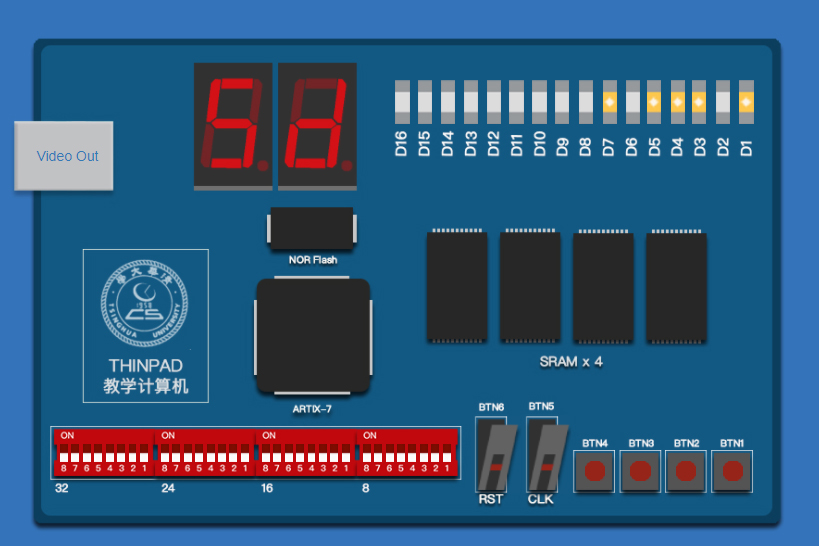
\includegraphics[width=0.5\textwidth]{hw_test.jpg}
\end{figure}

数码管和LED都停在了93,说明通过了全部93条测例。
}
}

\section{监控程序测试} {
监控程序有带TLB和不带TLB两个版本,由于带TLB的版本需要用到我们没有实现的tlbr和tlbp指令,所以我们只对不带TLB的版本进行了测试。

从这个阶段测试开始,用到了bootloader。编译生成的elf文件写入Flash,启动的入口地址指向片内ROM的bootloader代码的地址,由bootloader将$\mu$Core载入RAM并把控制权交给$\mu$Core,完成启动。

监控程序正常运行,执行R、D、A、G、T等交互指令会在串口中输出期望的信息。验证了基本指令的实现、基本异常处理(除TLB相关异常)的实现、Flash模块的实现、串口通信的实现的正确性。
}

\section{\boldsymbol{\mu}Core测试} {
%\section{$\mu$Core测试} {
$\mu$Core的作为教学系统,从简单到复杂共有8个阶段:\begin{enumerate}
	\item 完成boot过程,初始化中断处理和异常处理。
	\item 实现物理内存管理。
	\item 实现虚拟内存管理。
	\item 实现内核线程管理。
	\item 实现用户进程管理。
	\item 实现一个新的调度方法。
	\item 实现同步互斥功能。
	\item 加载用户系统,进入用户态。
\end{enumerate}

8个阶段加载完成后,证明$\mu$Core成功运行。

我们将$\mu$Core编译成elf烧入Flash中,由putty进行串口通信。按下重启键后,putty显示交互信息,最后停止在了一个交互环境。在交互环境中我们对sh、cat、pwd、hello等用户程序进行了测试,均正常执行。这个阶段进一步验证了所需要指令实现的正确性、异常处理的正确性,同时验证了TLB以及相关指令和异常实现的正确性。

下一步,我们对$\mu$Core的代码进行了修改,在向串口输出的语句后面增加向VGA输出的语句,以此实现将信息打印在屏幕上的效果。验证了VGA硬件模块实现的正确性,同时也验证了打印字符的软件模块(提供了向屏幕光标位置打印字符的接口,难点在于换行和滚屏)实现的正确性。
}


\section{u-boot测试} {
\subsection{基础工作} {
编译$\mu$Core,生成用于u-boot的镜像ucore.ub。
}
\subsection{以太网启动测试} {
将电脑与实验板用双绞线相连。下载并安装Windows下的TFTP服务端,设置好要用于文件共享的文件夹。将ucore.ub放入共享文件夹中。在putty中输入所需命令以启动$\mu$Core。在putty中可以看到u-boot的启动信息,之后又可以看到$\mu$Core的交互信息,证明启动成功。这个测试验证了以太网模块实现的正确性。
}
\subsection{usb启动测试} {
准备好只有一个分区的FAT32格式U盘。将ucore.ub置于其根目录。将U盘插入实验板的usb口。在putty中输入所需命令以启动$\mu$Core。在putty中可以看到u-boot的启动信息,之后又可以看到$\mu$Core的交互信息,证明启动成功。这个测试验证了usb模块实现的正确性。
}
}
	
\end{document}